\documentclass{article}
\usepackage{blindtext}
\usepackage[utf8]{inputenc}
\usepackage{polski}
 \usepackage{geometry} 
 \usepackage{graphicx}
\newgeometry{tmargin=3cm, bmargin=3cm, lmargin=3cm, rmargin=3cm}
\renewcommand{\figurename}{Wykres}
\title{Perceptron prosty oraz Adaline}
\date{11 październik 2017}
\author{Piotr Grzybowski}
 
\begin{document}
 
\maketitle
\newpage

\section{Opis problemu}
    Symulowanie działania bramek logicznych realizujących proste funkcje logiczne przy pomocy modeli matematycznych jako problem klasyfikacji binarnej.\\[0.3cm]
	Celem klasyfikacji binarnej jest \textit{zaklasyfikowanie}, czyli przypisanie każdego elementu z danego zbioru do dwóch rozłącznych kategorii. \\[0.3cm]     
	Rozważmy bramki logiczne, które mają dwa wejścia i jedno wyjście. Taka bramka działa jak klasyfikator binarny. Parze sygnałów wejściowych zostaje przypisana wartość zero lub jeden. (Przypisanie pary wejść do jednej z dwóch możliwych kategorii.)\\[0.3cm]
    W klasycznych bramkach logicznych wejścia jak i wartość realizowanej funkcji przyjmuje dyskretne wartości: zero lub jeden. Naszym zadaniem będzie zbudowanie, oraz wyuczenie modelu, który będzie poprawnie odzwierciedlał działanie funkcji także w przypadku gdy na wejściu pojawią się wartości ciągłe z pewnym odchyleniem $\epsilon$. Przykład działania bramki logicznej \textit{AND} przy $\epsilon = 0.05$. (0.95 \textit{AND} 0.05) = 0. \\[0.3cm]
    Zbiór danych za pomocą którego odbędzie się uczenie sieci neuronowej składać się będzie z uporządkowanych trójek $(x_1, x_2, y)$, gdzie $x_1, x_2$ to wartości sygnałów wejściowych do bramek logicznych, oraz $y$ jako wartość konkretnej funkcji logicznej dla podanych wejść. (Klasa do której możemy przypisać daną parę sygnałów wejściowych.)
    
    
\section{Proponowane rozwiązanie}
	Powyżej zaprezentowany problem zostanie rozwiązany przy użyciu prostej sieci neuronowej jako klasyfikatora binarnego. A dokładniej tylko pojedynczego neuronu w dwóch wersjach: pojedynczy perceptron prosty, oraz pojedyncza komórka Adaline.
	
	\subsection{Sieć neuronowa}
	Każdy z neuronów składa się z: 
	\begin{itemize}
		\item Wektora wag o długości liczbie sygnałów wejściowych. Każdemu sygnałowi wejściowemu $x_i$, odpowiada dokładnie jedna kolejna waga $w_i$. Symbolicznie $W = [x_1, ..., x_N]$, gdzie N to liczba sygnałów wejściowych do neuronu.
		\item Stałej zwanej "biasem". Liczba rzeczywista.
		\item Funkcji aktywacji, według której obliczana jest wartość wyjścia neuronów w sieci neuronowej.
	\end{itemize}
    Wartość wyjścia neuronu jest liczona w sposób następujący (\textit{g} - funkcja aktywacji)
    \begin{equation}
    		Output = g(x^Tw + b)
    \end{equation}
    
    Podczas rozwiązywania zadania zostaną zbadane dwa typy neuronów. Perceptron prosty oraz komórka Adaline. Ich struktura jest taka sama, jednakże różnią się procedurą uczenia. Sposoby te omówione zostaną poniżej.
    
    \newpage
    \subsection{Uczenie perceptronu prostego}
    Uczenie sieci realizowane jest poprzez aktualizację wag perceptronu dla każdego przypadku treningowego w każdej kolejnej iteracji uczenia. 
    \begin{equation}
    w_i^{t+1} = w_i^t + \mu * \delta * x_i
    \end{equation}
    gdzie:
    \begin{itemize}
        \item $w_i^{t+1}$ wartość \textit{i-tej} wagi w czasie $t+1$.
        \item $w_i^t$ - aktualna wartość $w_i$.
        \item $\mu$ - stała uczenia.
        \item $x_i$ - wartość i-teg wygnału wejściowego.
    \end{itemize}
    
    W przypadku perceptronu prostego błąd $\delta$ definiuje się jako różnicę między wartością oczekiwaną a wartością funkcji aktywacji perceptronu:
    \begin{equation}
    \delta = E - P
    \end{equation}
    gdzie:
    \begin{itemize}
    	\item E - wartość oczekiwana,
    	\item P - wartość predykowana
    \end{itemize}
    Ostatecznie procedura aktualizacji wag w każdym kroku będzie wyglądać następująco:
     \begin{equation}
        w_i^{t+1} = w_i^t + \mu * (E-P) * x_i
     \end{equation}
    
    \subsection{Uczenie komórki Adaline}
    Uczenie sieci realizowane jest poprzez aktualizację wag perceptronu dla każdego przypadku treningowego w każdej kolejnej iteracji uczenia w podobny sposób jak dla perceptronu prostego. Jednakże zamiast błędu dyskretnego $\delta$ będzie brany gradient błędu średniokwadratowego.
    \begin{equation}
    w_i^{t+1} = w_i^t + \mu * \nabla_{w_i} \delta * x_i
    \end{equation}
    gdzie:
    \begin{itemize}
        \item $w_i^{t+1}$ wartość \textit{i-tej} wagi w czasie $t+1$.
        \item $w_i^t$ - aktualna wartość $w_i$.
        \item $\mu$ - stała uczenia.
        \item $x_i$ - wartość i-teg wygnału wejściowego.
    \end{itemize}
    Różnicą będzie w postaci funkcji błędu. Skorzystamy tutaj z błędu średniokwadratowego. Wartością błędu będzie różnica wartości oczekiwanej oraz wartości pobudzenia neuronu. W przypadku perceptronu prostego do wyliczenia błędu aplikowana jeszcze była funkcja aktywacji do pobudzenia.
    \begin{equation}
    \delta_i = d_i - x^Tw 
    \end{equation}
    
    \begin{equation}
     \delta_i^2 = (E_i - \Sigma_{i=1}^{N} x_i*w_i )^2 
     \end{equation}
     
     \begin{equation}
     \frac{\partial \delta_i^2}{\partial w_i} = 2 * \delta_i * \frac{\partial \delta_i}{\partial w_i}
     \end{equation}
    gdzie:
    \begin{itemize}
    	\item E - wartość oczekiwana,
    	\item P - wartość predykowana
    \end{itemize}
    
	\newpage
	\section{Zbiór danych}
	Do przygotowania zbioru danych został napisany generator, żeby w prosty sposób móc otrzymać zadaną liczbę przykładów w zbiorze. Zbiór generuje się w zależności od liczby przypadków oraz odchylenia epsilon. Odchylenie posłuży nam do zamodelowania logiki rozmytej. Przykładowo dla $\epsilon = 0.1$ i dla funkcji logicznej AND, pozytywne sygnały wejściowe przyjmą wartości z zakresu [0.9, 1] a negatywne z zakresu [0, 0.1].
	\newpage
	\section{Badania}
	Wyniki uczenia i jakości predykcji neuronów przy różnych parametrach o różnej wielkości zbioru danych.
	\subsection{Adaline}
	    Wymagana liczba epok do wyuczenia Adaline w zależności od wielkości zbioru uczącego na wykresie 1 poniżej:
	    
	\begin{figure}[h]

		\centering
		\caption{}
		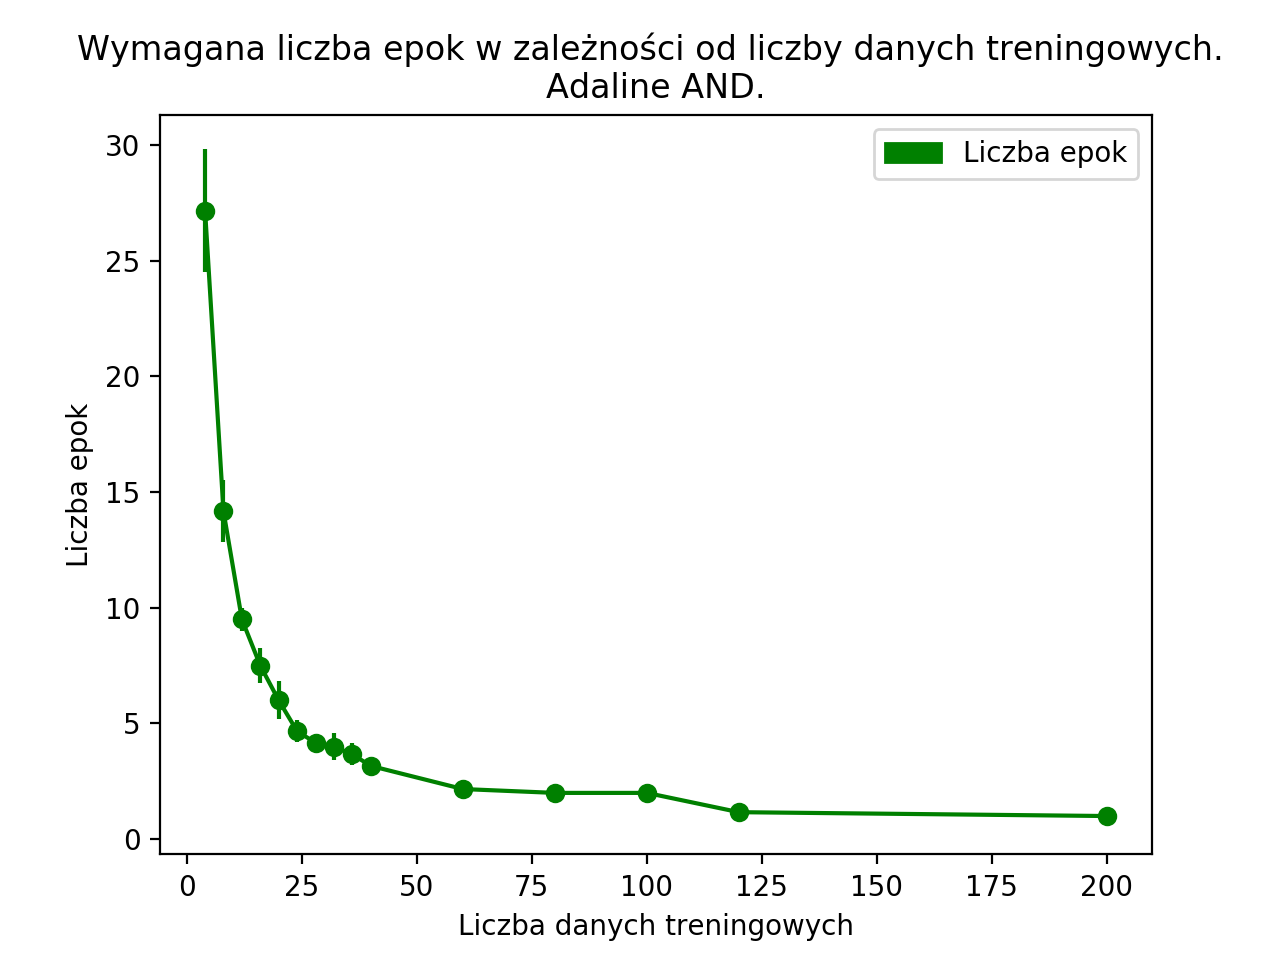
\includegraphics[width=0.5\textwidth]{epoki_dane_adaline_and.png}
		
	\end{figure}	 
	Na podstawie powyższego wykresu wyraźnie widać, że wraz ze wzrostem liczebności zbioru treningowego maleje liczba epok wymaganych do wyuczenia Adaline. Dzieje się tak dlatego, że podczas jednej epoki dostosowujemy wagi więcej razy.\\[0.5cm] 
	
	Wymagana liczba epok do wyuczenia Adaline w zależności od stałej uczenia na wykresie 2 poniżej:
	
	\begin{figure}[h]

		\centering
		\caption{}
		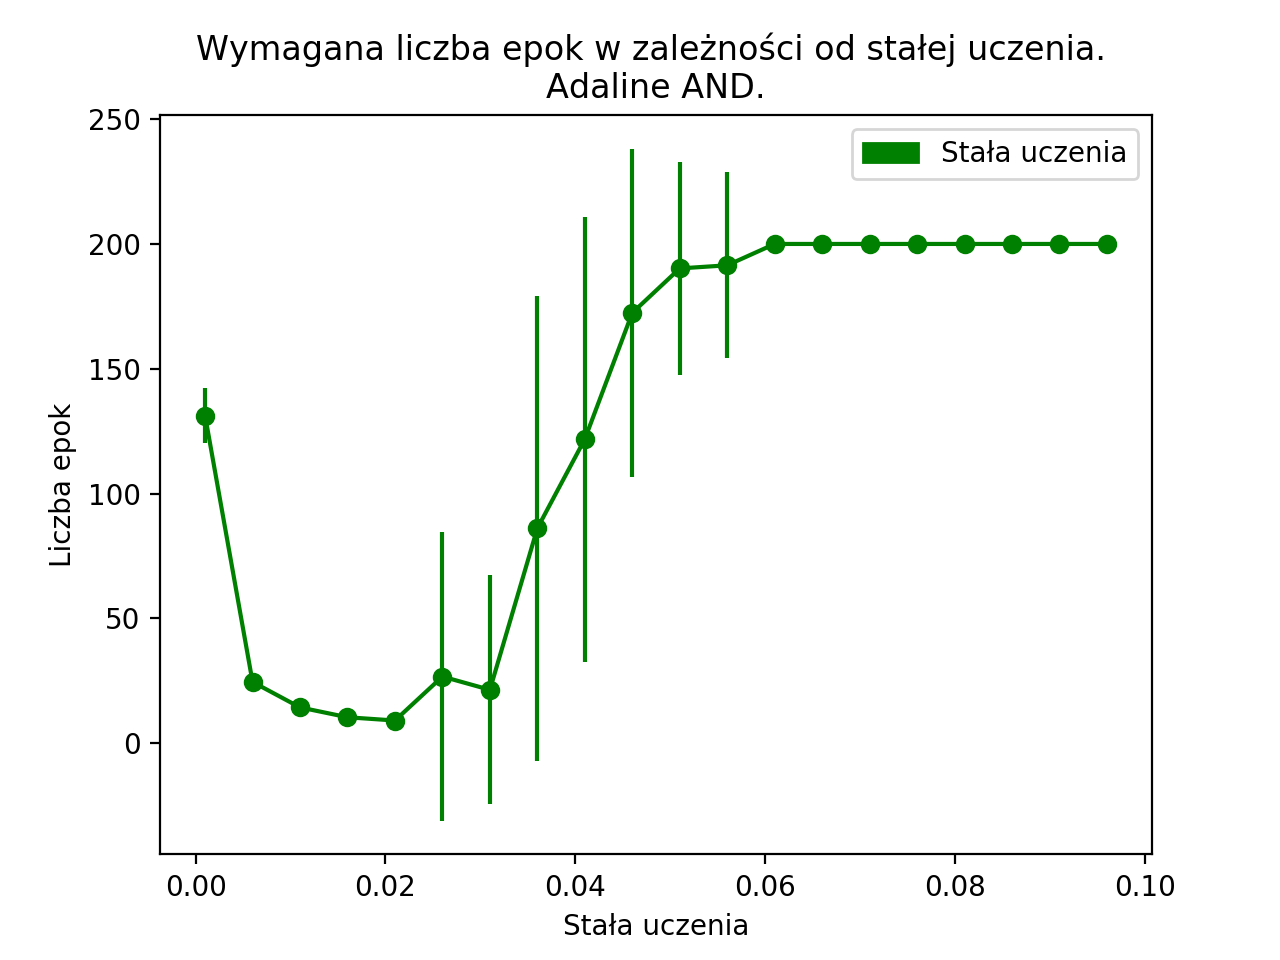
\includegraphics[width=0.5\textwidth]{epoki_rate_adaline.png}
		
	\end{figure}   
	Na podstawie powyższego wykresu wyraźnie widać, że zależność liczby epok od kroku uczenia ma pewne minimum. Istnieje taki zakres wartości stałej uczenia w której Adaline wyucza się najszybciej. Oznacza to, że wartość kroku uczenia nie może być ani zbyt mała ani zbyt duża.
	\newpage
	Wymagana liczba epok do wyuczenia Adaline w zależności od zakresu initializowanych wag na wykresie 3 poniżej:
	
	\begin{figure}[h]

		\centering
		\caption{}
		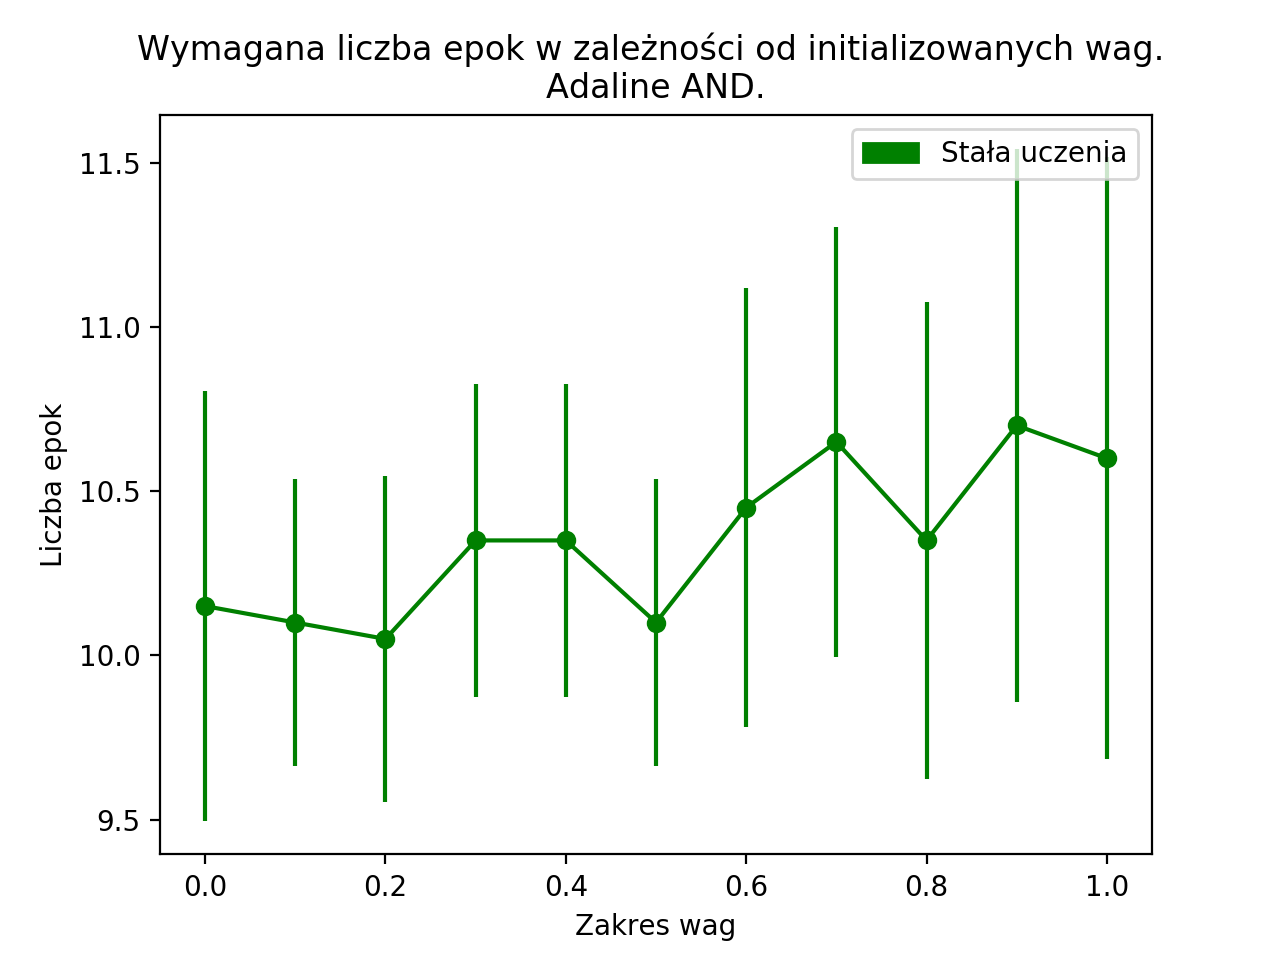
\includegraphics[width=0.5\textwidth]{epoki_wagi_adaline_and.png}
		
	\end{figure}   
	Zakres wag początkowych nie ma większego znaczenia w tym przypadku. Każdy z zakresów charakteryzuje się dużą wariancją i brakuje stabilnych wyników.
\newpage
	\subsection{Perceptron}
	\subsubsection{Funkcja aktywacji unipolarna}
	Wymagana liczba epok do wyuczenia perceptronu prostego dla funkcji aktywacji unipolarnej w zależności od wielkości zbioru uczącego na wykresie 4 poniżej:
	\begin{figure}[h]
		\centering
		\caption{}
		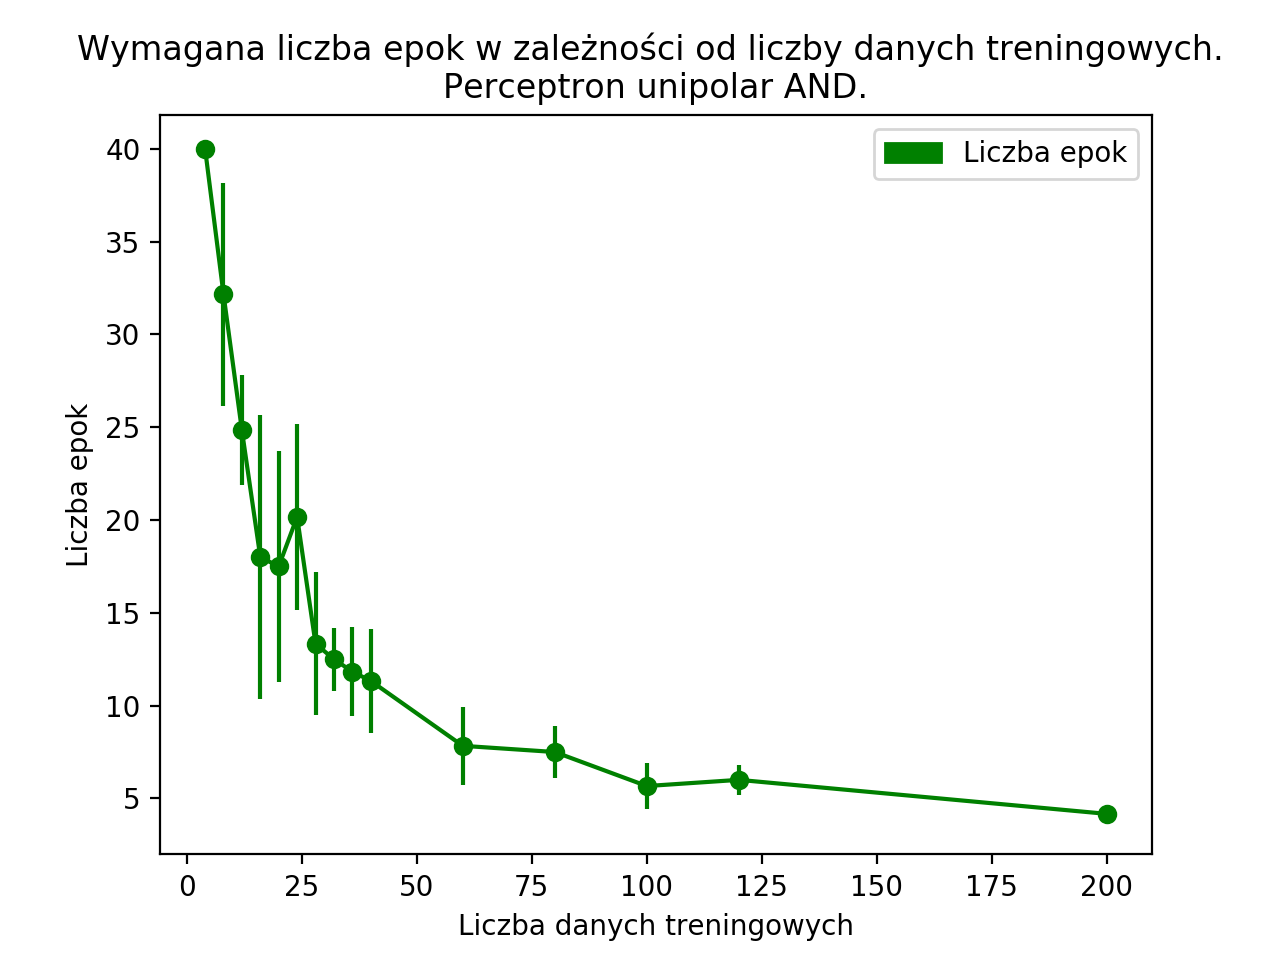
\includegraphics[width=0.5\textwidth]{epoki_dane_perceptron_unipolar_and.png}
	\end{figure}
	
	Wnioski do tego wykresu są analogiczne do wykresu 1. Jak w przypadku Adaline.\\[0.5cm]
	
	Wymagana liczba epok do wyuczenia perceptronu prostego dla funkcji aktywacji unipolarnej w zależności od wielkości zbioru uczącego na wykresie 5 poniżej:
	
	\begin{figure}[h]
		\centering
		\caption{}
		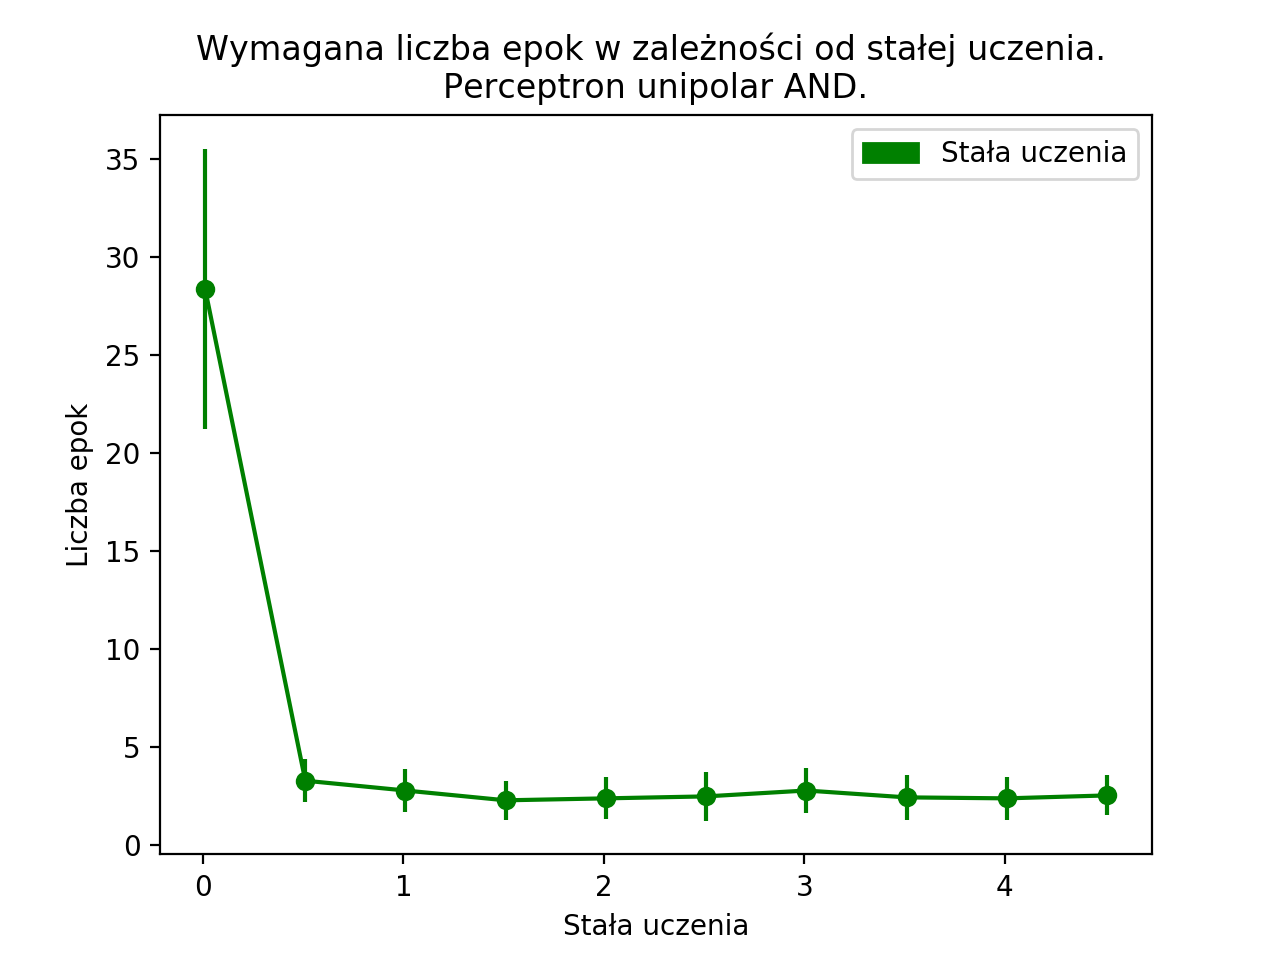
\includegraphics[width=0.5\textwidth]{epoki_rate_perceptron_unipolar.png}
	\end{figure}
	
	Uczenie perceptronu nie ma nic wspólnego z algorymem gradientu prostego. Nie ma więc znaczenia jak duża będzie stała uczenia. Wagi będą po prostu przeskalowane.
	\newpage
		Wymagana liczba epok do wyuczenia perceptronu prostego dla funkcji aktywacji unipolarnej w zależności od wielkości zbioru uczącego na wykresie 6 poniżej:
	
	\begin{figure}[h]
		\centering
		\caption{}
		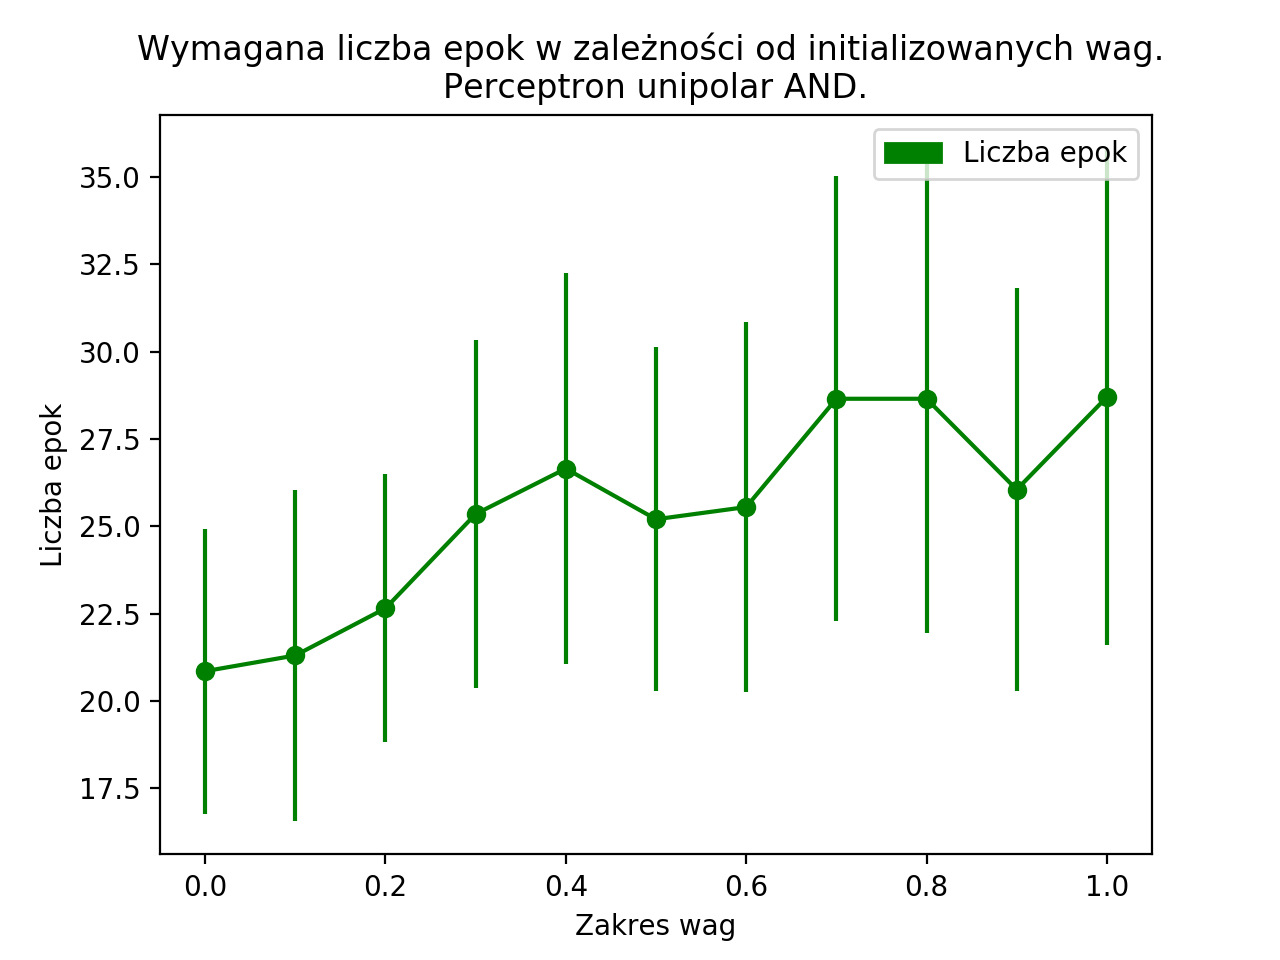
\includegraphics[width=0.5\textwidth]{epoki_wagi_perceptron_unipolar.png}
	\end{figure}
	
	Wyniki są obarczone dużą wiariancją. Dla bardzo małego zbioru treningwego można wywnioskować pewien trend rosnący, jednakże przy większym zbiorze treningowym, zakres initializowanych wag nie wpływa na szybkość uczenia.
	\newpage
	\subsubsection{Funkcja aktywacji bipolarna}
	Wymagana liczba epok do wyuczenia perceptronu prostego dla funkcji aktywacji bipolarnej w zależności od wielkości zbioru uczącego na wykresie 7 poniżej:
	\begin{figure}[h]
		\centering
		\caption{}
		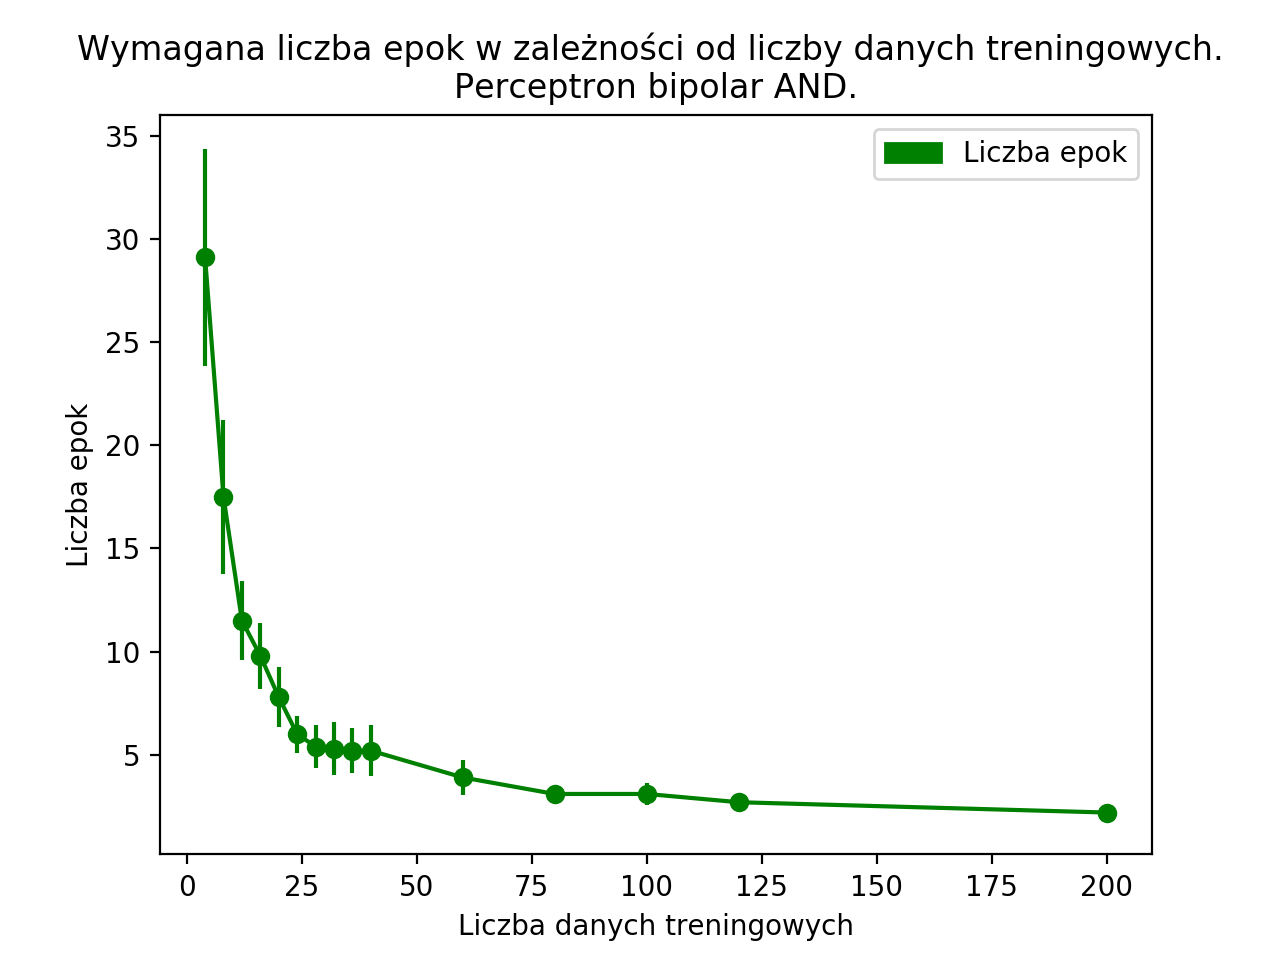
\includegraphics[width=0.5\textwidth]{epoki_date_perceptron_bipolar.png}
	\end{figure}

Wnioski do tego wykresu są analogiczne do wykresu 1. Jak w przypadku Adaline.\\[0.5cm]

	Wymagana liczba epok do wyuczenia Adaline w zależności od zakresu initializowanych wag na wykresie 8 poniżej:
	
	\begin{figure}[h]

		\centering
		\caption{}
		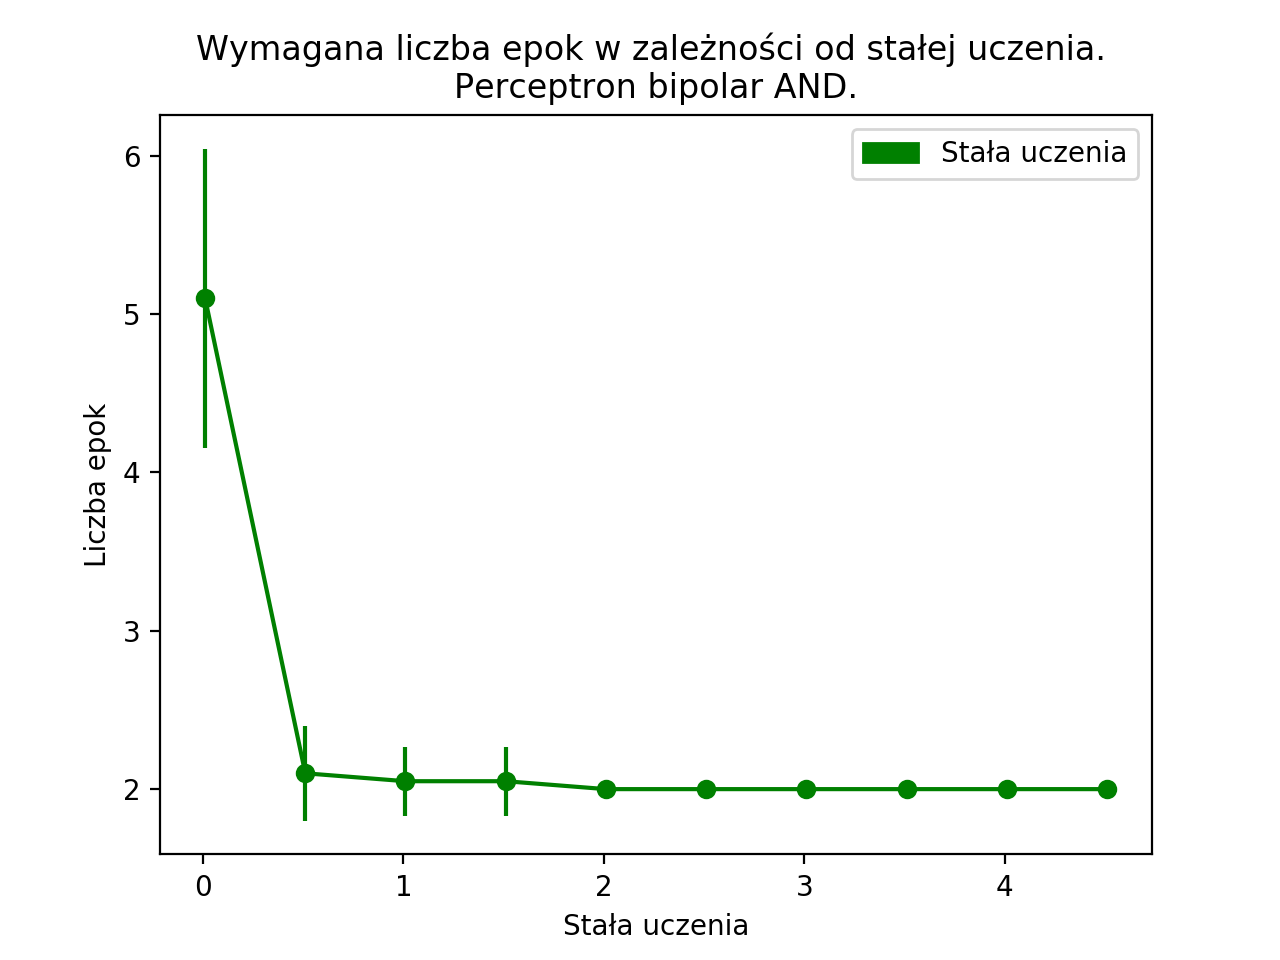
\includegraphics[width=0.5\textwidth]{epoki_rate_perceptron_bipolar.png}
		
	\end{figure}  
	Uczenie perceptronu nie ma nic wspólnego z algorymem gradientu prostego. Nie ma więc znaczenia jak duża będzie stała uczenia. Wagi będą po prostu przeskalowane.
		\newpage
	Wymagana liczba epok do wyuczenia Adaline w zależności od zakresu initializowanych wag na wykresie 9 poniżej:
	
	\begin{figure}[h]

		\centering
		\caption{}
		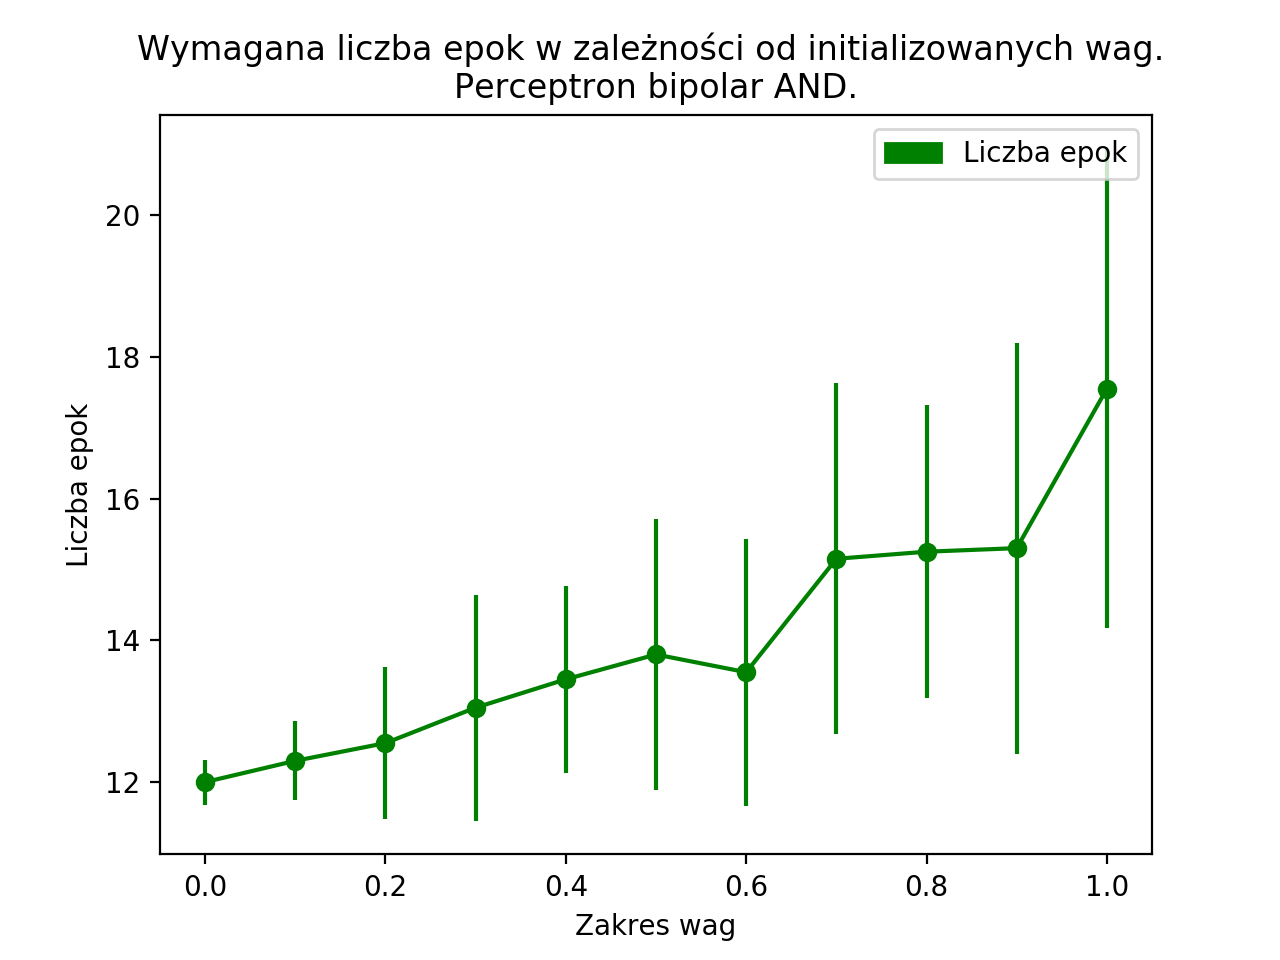
\includegraphics[width=0.5\textwidth]{epoki_wagi_perceptron_bipolar.png}
		
	\end{figure}   
	
	\subsection{Przykładowy wykres błędu w trakcie uczenia}
	Wykres błędu w zależności od epoki na wykresie 10 poniżej:
	
	\begin{figure}[h]
		\centering
		\caption{}
		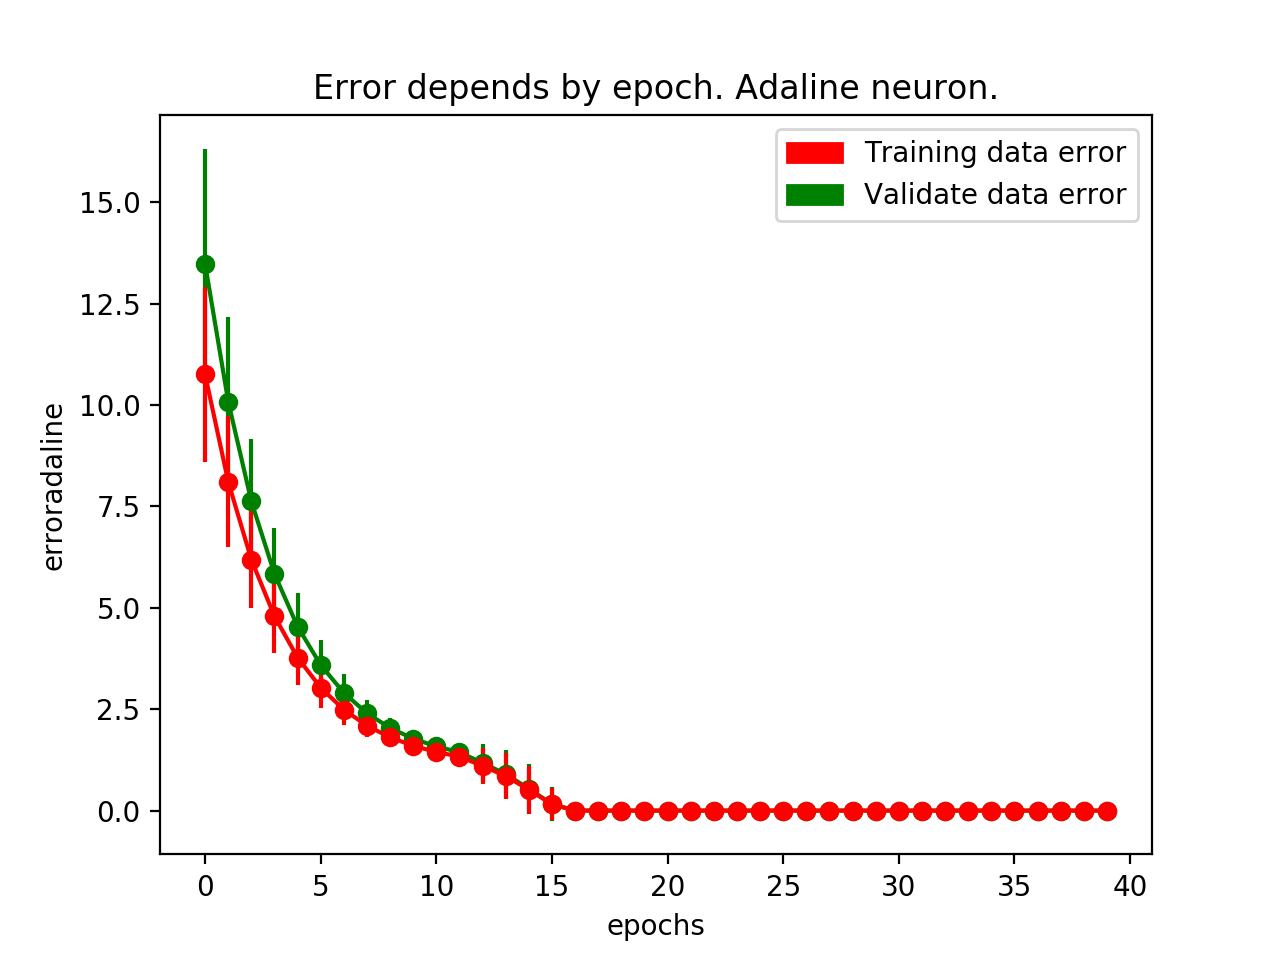
\includegraphics[width=0.5\textwidth]{adaline_and.png}
		
	\end{figure}  
\newpage	
	\section{Podsumowanie}
	
	
	Na podstawie przeprowadzonych badań w trakcie ćwiczenia zauważono, że w przypadku Adaline krok uczenia ma znaczenie w przeciwieństwie do perceptronu prostego. Dla Adaline wartość kroku uczenia nie może być ani zbyt mała ani zbyt duża. Gdy będzie zbyt mała będzie potrzeba zbyt wielu epok aby wyuczyć model, a w przypadku dużego kroku uczenia mamy do czynienia ze zjawiskiem eksplodującego gradientu. Dla perceptronu prostego stała uczenia nie może być zbyt mała z tego samego powodu, jednakże w przypadku jak będzie ona duża to nie wływa ona na jakość uczenia.\\[0.3cm]
	
Dla obydwóch modeli, liczba wymaganych epok maleje wraz z liczbą elementów w zbiorze treningowym.\\[0.3cm]
	
Dla obydwóch modeli zakres wartości wag początkowych nie miał większego znaczenia w szybkości uczenia. Jedynie w przypadku bardzo małego zbioru treningowego, można zauważyć pewien trend. Dla bardzo małego zbioru treningowego, potrzebnych jest mniej epok gdy wagi są zbliżone do zera. \\[0.3cm]

Obydwa modele nie radzą sobie z problemami nieseparawoalnymi liniowo.\\[0.3cm]


\end{document}

